\chapter{The JUNO detector}
The Jiangmen Underground Neutrino Observatory~(JUNO) is a multi-functional neutrino experiment project in southern China, as shown in Fig.~\ref{fig:juno_site}. The Central Detector~(CD) is located in a laboratory \SI{700}{m} underground~\cite{muon207}. Its excellent energy resolution and relatively large effective volume provide an exciting opportunity to address many important issues in the fields of neutrino and astroparticle physics. As evidenced in Tab.~\ref{tab:juno_core}, there are two nuclear power plants, Yangjiang~(YJ) and Taishan~(TS), at around \SI{53}{km} away from the JUNO detector. After 2000 days of data taking, the measurement result of NMO can be obtained with a confidence level of $3\sigma$, as shown in Fig.~\ref{fig:juno_nmo_2000}.

\begin{figure}[htbp]
	\centering
	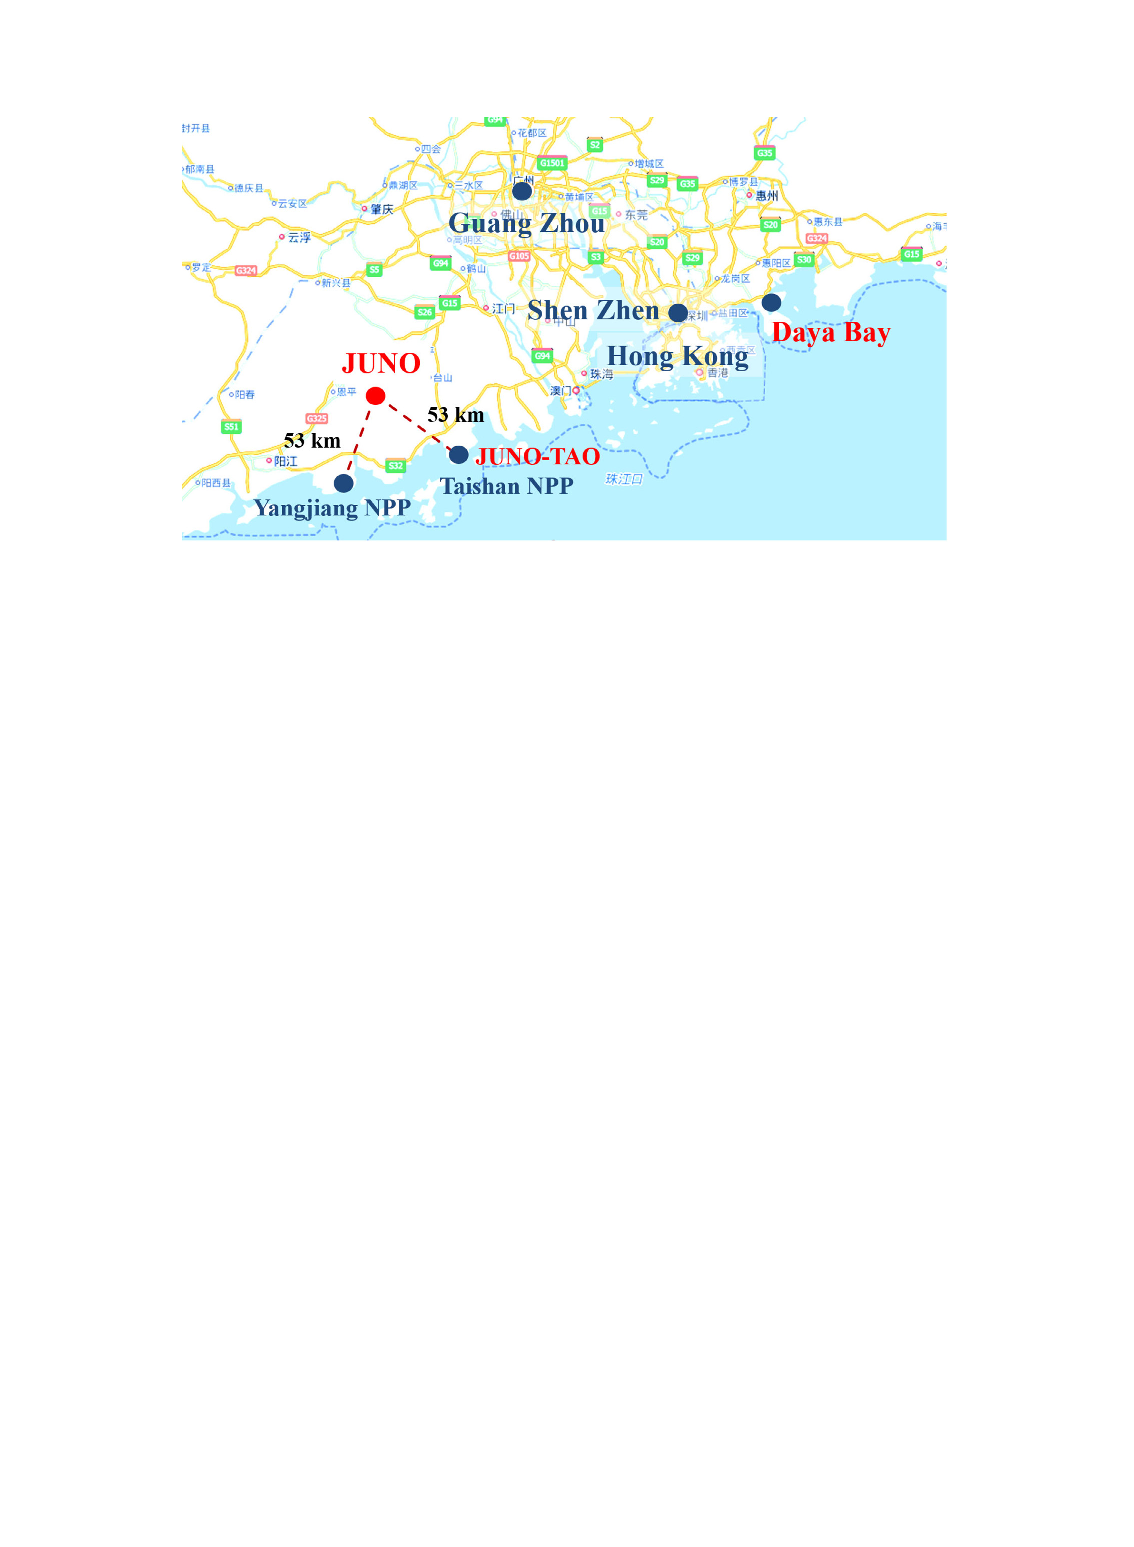
\includegraphics[width=0.7\textwidth]{junoDetector/location.pdf}
	\caption{The location of JUNO~\cite{muon207}: Jinji, Kaiping city, Jiangmen city, Guangdong province, China. Its geographical location is $112^{\circ}31^{\prime}05^{\prime\prime}~\mathrm{E}$ and $22^{\circ}07^{\prime}05^{\prime\prime}~\mathrm{N}$.}
	\label{fig:juno_site}
\end{figure}

\begin{table}[htbp]
	\centering % 表格居中
	\caption{The power of the reactor core and the baseline distance, the data comes from~\cite{juno_yellow_book}}
	\label{tab:juno_core}
	\begin{tabular}{cccccccc}
		\toprule % 顶线
		\textbf{Cores}     & YJ-C1 & YJ-C2 & YJ-C3 & YJ-C4 & YJ-C5 & YJ-C6 \\
		\midrule
		Power~(\si{GW})    & 2.9   & 2.9   & 2.9   & 2.9   & 2.9   & 2.9   \\
		Baseline~(\si{km}) & 52.75 & 52.84 & 52.42 & 52.51 & 52.12 & 52.21 \\
		\addlinespace
		\textbf{Cores}     & TS-C1 & TS-C2 & TS-C3 & TS-C4 & DYB   & HZ    \\
		\midrule
		Power~(\si{GW})    & 4.6   & 4.6   & 4.6   & 4.6   & 17.4  & 17.4  \\
		Baseline~(\si{km}) & 52.76 & 52.63 & 52.32 & 52.20 & 215   & 265   \\
		\bottomrule
	\end{tabular}
\end{table}

\begin{figure}[htbp]
	\centering
	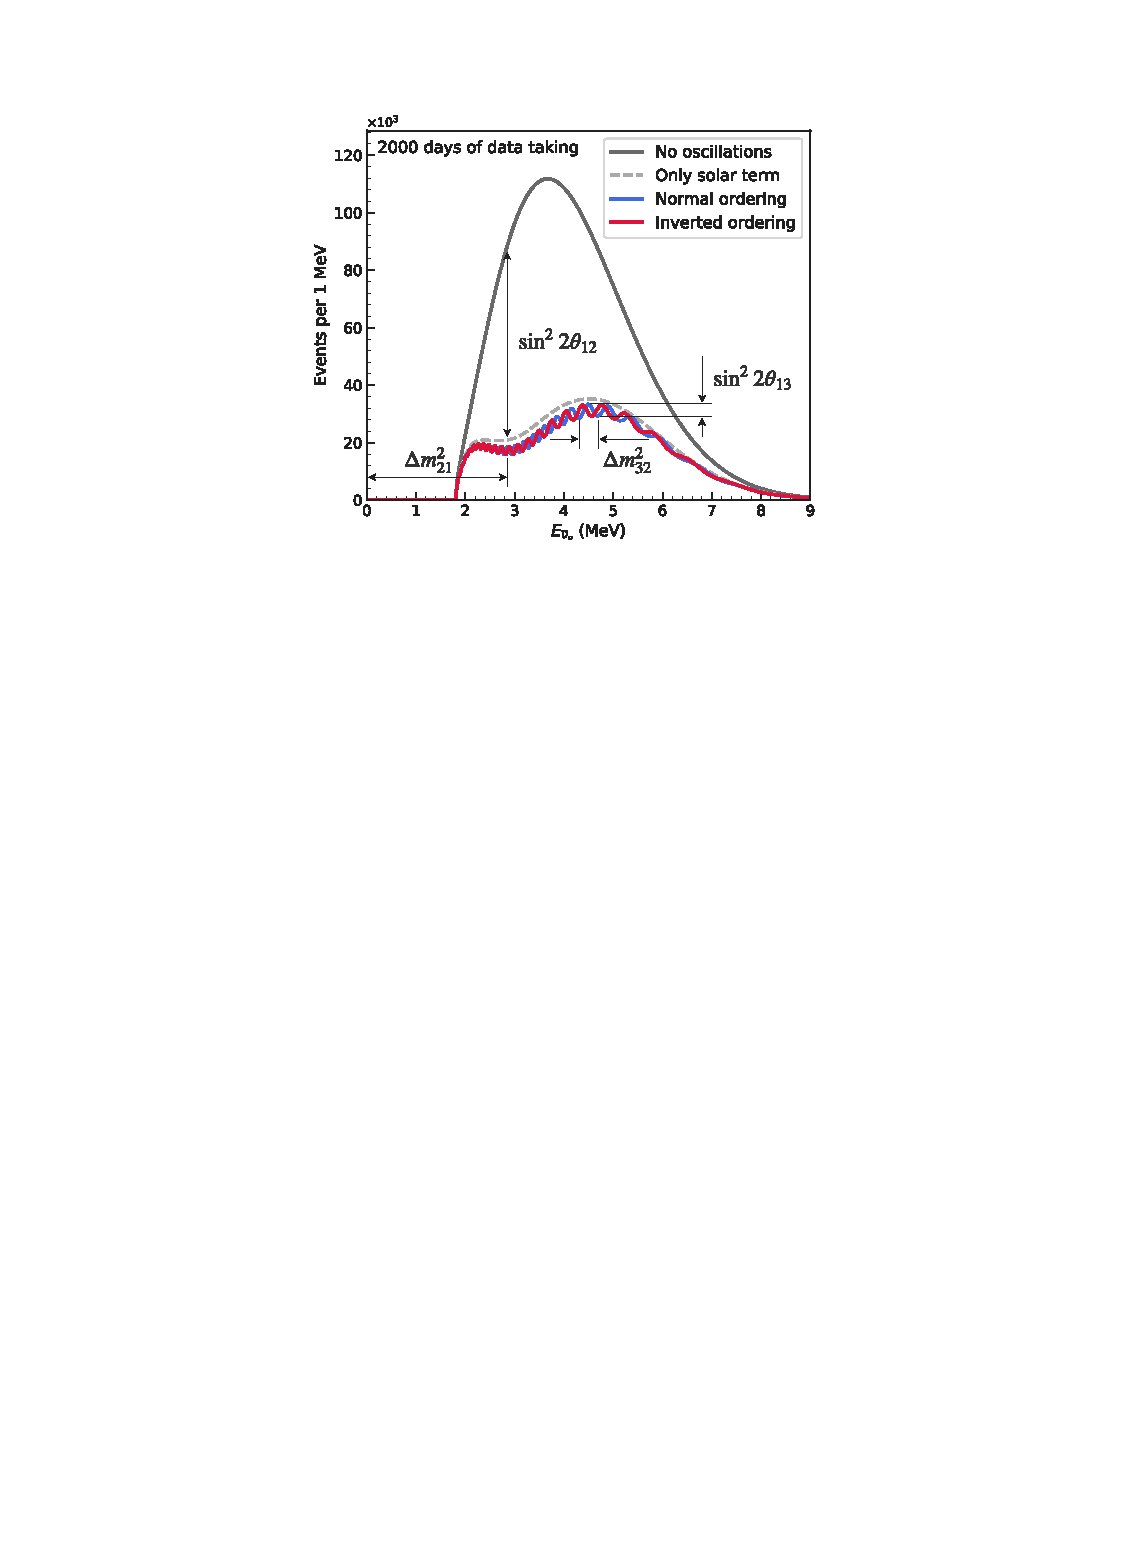
\includegraphics[width=0.5\textwidth]{junoDetector/nmo_2000day.pdf}
	\caption{The sensitivity of NMO measurement at JUNO after 2000 days of data taking based on simulation. Four oscillation parameters are depeended on~\cite{muon207}.}
	\label{fig:juno_nmo_2000}
\end{figure}

\section{The structure of JUNO detector}
The JUNO detector is composed of CD, a water Cherenkov detector based on the water pool~(WCD), and a Top Tracker~(TT), as illustrated in Fig.~\ref{fig:juno_cd_structure}.
\begin{figure}[htbp]
	\centering
	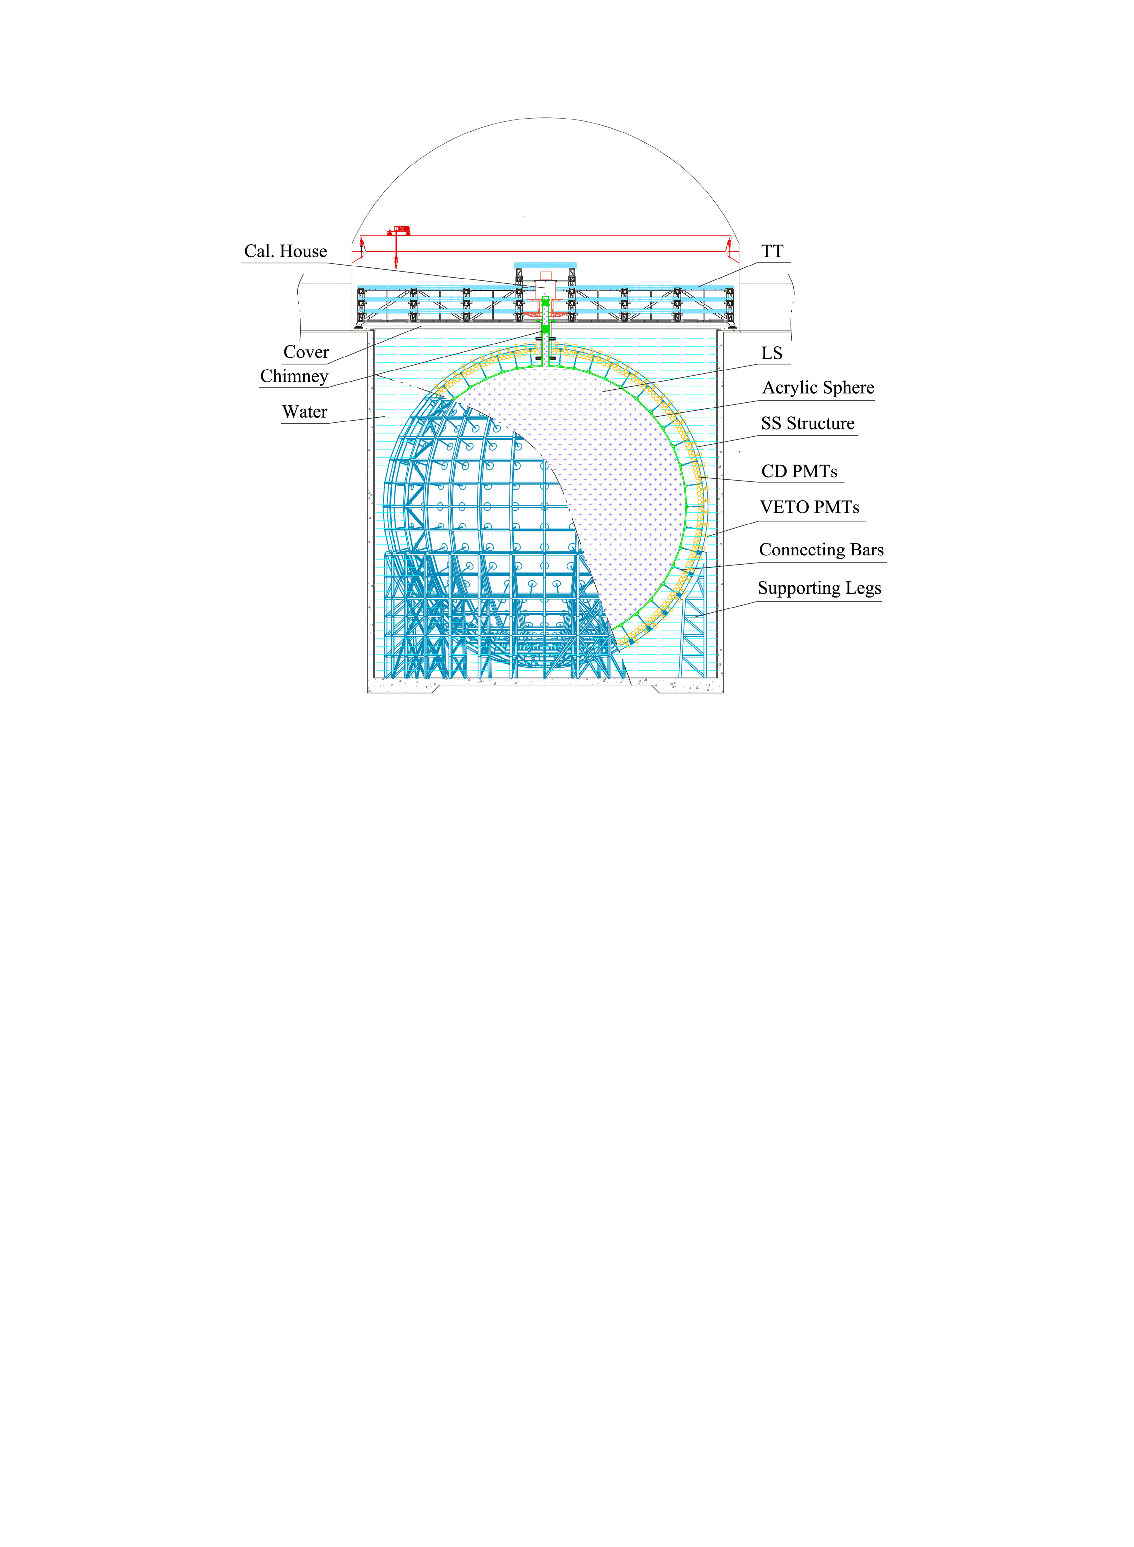
\includegraphics[width=0.6\textwidth]{junoDetector/structure.pdf}
	\caption{The structure of JUNO detector. The figure comes from~\cite{muon207}}
	\label{fig:juno_cd_structure}
\end{figure}
\subsection{The Central Detector}
The Central Detector consists of an acrylic spherical shell with a diameter of \SI{35.4}{m} and a thickness of \SI{12}{cm}, which is filled with 20 kton of liquid scintillator. It is engineered to attain an energy resolution of $\frac{\SI{3}{\%}}{\sqrt{E}}$ to facilitate the measurement of NMO. To detect the photons emitted due to the energy deposited by particles, 17,612 20-inch and 25,600 3-inch photomultiplier tubes~(PMTs), more detailed information in Tab.~\ref{tab:juno_pmt}, are mounted on a spherical structure with a radius of \SI{19.5}{m}. This setup achieves a photocathode coverage rate of over \SI{75}{\%}. Ultra-pure water is filled between the PMT and the acrylic to shield the radioactive background from the surface of the PMT. The entire CD detector is immersed in a cylindrical water pool to shield the radioactive background from the surrounding rocks, etc. At the same time, the water pool, as a Cherenkov detector, is equipped with 1,600 20-inch PMTs, enabling the detection of \SI{99.8}{\%} of cosmic muons. To avoid the interference of the geomagnetic field, a set of 32 circular coils surrounding the detector is designed to keep the residual magnetic field in the PMT area of CD less than \SI{0.05}{G} and that in WCD below \SI{0.1}{G}~\cite{muon207}.

\begin{table}[htbp]
	\centering % 表格居中
	\caption{The summary of PMTs used in JUNO CD, the data comes from~\cite{muon207,PMT-3inch,JUNO:2022hlz}}
	\label{tab:juno_pmt}
	\begin{tabular}{cccccccc}
		\toprule % 顶线
		    & Size~(\si{inch}) & Type       & Number & Manufacturer                               \\
		\midrule % 中线
		CD  & 20               & MCP-PMT    & 12612  & Northern Night Vision Technology Co.       \\
		    &                  & Dynode-PMT & 5000   & Hamamatsu Photonics K. K.                  \\
		    & 3                & SPMT       & 25600  & Hainan Zhanchuang Photonics Technology Co. \\
		WCD & 20               & MCP-PMT    & 2400   & Northern Night Vision Technology Co.       \\
		\bottomrule % 底线
	\end{tabular}
\end{table}

\subsection{The Top Tracker}
